\documentclass[a4paper,12pt]{article}
\usepackage{polski}
\usepackage[utf8]{inputenc}
\usepackage[OT4]{fontenc}
\usepackage{mathtools}
\usepackage{float}
\usepackage{graphicx}
\usepackage{multirow}

\newcommand{\h}[1]{\noindent \bf #1 \rm \\ \noindent}
\newcommand{\italic}[1]{\it #1 \rm}


\begin{document}

\begin{center}
	\LARGE
	Sieci Komputerowe \\
	\large
	LABORATORIUM 1 
\end{center}
\vspace{1cm}
	
\h{Komenda "ipconfig":}
Komenda pozwalająca na wyświetlenie danych nt konfiguracji sieciowej komputera lub jej zmianę. Może one być użyta chociażby do sprawdzenia aktualnie przypisanego urządzeniu adresu IPv4. Na systemach UNIX jej odpowiednikiem jest \it ifconfig\rm.

\begin{figure}[H]
	\centering
	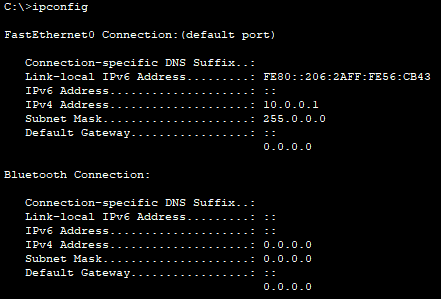
\includegraphics[width=10cm]{fig1.png}
	\caption{Efekt skorzystania z komendy \it ipconfig\rm.}
\end{figure}

\noindent
Do komendy \it ipconfig \rm możemy dodać również parametry, zmieniające jej działanie:
\begin{itemize}
	\item \italic{brak parametru} - wyświetlenie skrótowej informacji nt konfiguracji sieciowej
	\item \italic{/all} - wyświetla szczegółowe informacje na temat konfiguracji sieciowej (w tym adres MAC)
	\item \italic{/release} - zwalnia wszystkie adresy IP przydzielone do karty sieciowej
	\item \italic{/renew} - pobiera nowe adresy IP dla karty sieciowej (wymaga aktywnego DHCP)
	\item \italic{/flushdns} - usuwa informacje na temat nazw domen z pamięci serwera DNS 
	\item \italic{displaydns} - wyświetla nazwy domen zawarte w pamięci serwera DNS
	\item \italic{registerdns} - odświeża i aktualizuje informacje o nazwach domen w serwerze DNS
\end{itemize}

\h{Komenda "ping":}
Komenda pozwalająca na diagnozowanie połączenia sieciowego między dwoma urządzeniami w sieci. Badanie polega na przesłaniu kolejno 4 pakietów ICMP z jednego urządzenia i oczekiwanie na odpowiedź z drugiego. Czas między wysłaniem pakietu a otrzymaniem odpowiedzi nazywamy czasem odpowiedzi czy też czasem ping.
	
\begin{figure}[H]
	\centering
	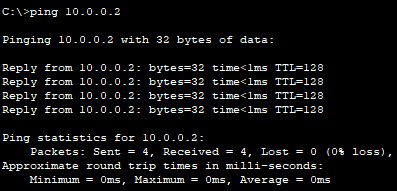
\includegraphics[width=10cm]{fig2.png}
	\caption{Efekt skorzystania z komendy \it ping\rm.}
\end{figure}	

\noindent
Za pomocą parametrów można dostosować ilość wysyłanych pakietów, czas oczekiwania na odpowiedź oraz rozmiar pakietów. Najczęściej używanymi są:
\begin{itemize}
	\item \italic{-n [ilość]} - ustala ilość pakietów które mają zostać przesłane
	\item \italic{-l [ilość]} - ustala wielkość pakietów
	\item \italic{-w [czas msek]} - określa maksymalny czas oczekiwania na odpowiedź
	\item \italic{-a} - nastąpi próba identyfikacji nazwy z serwera DNS
\end{itemize}

\noindent
Zamiast adresu IPv4 odbiorcy mnożna wpisać nazwę hosta, która następnie zostanie rozpoznana przez DNS.\\

\h{Protokół ICMP:}
Protokół ICMP (Internet Control Message Protocol) to protokół warstwy sieciowej, który jest używany do przesyłania wiadomości diagnostycznych i sterujących w sieciach IP. Często jest stosowany w diagnozowaniu problemów z siecią. Jego działanie polega na przesyłaniu wiadomości ICMP z między hostami, a następnie oczekiwaniu na odpowiedź.\\

\h{Komenda "tracert":}
Komenda pozwalająca na prześledzenie ścieżki pomiędzy hostami. Wyświetli ona informacje o wszystkich routerach przez które należy przejść, aby dotrzeć do hosta (pokaże dane o ścieżce do hosta). Jest to narzędzie oparte o wiadomości ICMP. Pozwala ono ustalić w łatwy sposób w którym punkcie ścieżki występuje problem z transmisją.

\begin{figure}[H]
	\centering
	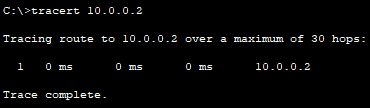
\includegraphics[width=10cm]{fig3.png}
	\caption{Efekt skorzystania z komendy \it tracert\rm.}
\end{figure}

Do komendy \italic{tracert} można dodać parametr zmieniający jej działanie:
\begin{itemize}
	\item \italic{-d} - wyłącza konwersję adresów na nazwy hostów (DNS).
	\item \italic{-h [ilość]} - ustala maksymalną ilość skoków, z których ma składać się ścieżka
\end{itemize}
	
\end{document}